% !TEX TS-program = LuaLaTeX

\PassOptionsToPackage{hyperref}{urlcolor=black}
\documentclass{internoise2026-wr}
\usepackage{booktabs,refstyle,siunitx}
\usepackage[style=numeric-comp,sorting=none,maxnames=99]{biblatex}
\defbibheading{bibliography}[\refname]{%
  \section*{\MakeUppercase{#1}}}
\DeclareFieldFormat{labelnumberwidth}{#1.}
\setlength{\biblabelsep}{0.5em}
\bibliography{acoustics,wspr-conf}

\begin{document}

\title{Introducing aubellhop: a modern Python interface to the Bellhop underwater acoustics ray tracing tool}

\maketitle

  \begin{flushleft}
    William S.P. Robertson,\markpresenting{1}
    Mandar Chitre,\markinstitution{2}
    Chung T.C. Fang,\markinstitution{1}
    Anthony C. Zander\markinstitution{1}

    \correspondingpresentingemail{will.robertson@adelaide.edu.au}

    \begin{multicols}{2} % <= choose the number of columns
    \institution[1]{%
      School of Electrical and Mechanical Engineering\\
      Adelaide University\\
      SA, Australia\\
    }
    \institution[2]{%
      Acoustic Research Laboratory,\\
      Tropical Marine Science Institute\\
      National University of Singapore\\
      Singapore
    }
    \end{multicols}
  \end{flushleft}

\smallskip
\begin{abstract}
Bellhop is widely used for modelling underwater acoustic propagation using ray/beam-tracing. As part of The Acoustics Toolbox, Bellhop was written in Fortran by Michael B. Porter and colleagues, as part of a suite of open source underwater acoustics modelling tools, and others have reimplemented it in C++/CUDA for multithreaded operation. Interfaces to Bellhop have been developed for several languages, including Matlab, Python, and Julia, but these tools sometimes only provide access to a subset of Bellhop's features, and often assume that the Bellhop executable is already installed. This paper introduces a modern Python interface to Bellhop, which can be used both by users who wish to run Bellhop simulations, or by developers who wish to adapt or extend the Bellhop codebase. As with the Julia interface, the Bellhop executable is included in the installation. Features of the package include: a comprehensive test suite with coverage reports against both Python and Fortran sources; detailed, online documentation of the Fortran and Python sources; automatic code quality checking as part of the repository workflows; and a series of tutorials demonstrating the main use cases of the simulation tools.
\end{abstract}

\section{Introduction}
\label{sec:intro}

Bellhop is an open source Fortran program for calculating underwater acoustic phenomena \cite{porter2025-foa} using ray tracing and beam tracing algorithms (\Figref{erays}).
It is written and maintained by Michael B. Porter, with early development in the 1980s (first release 1983 with Homer Bucker, Naval Ocean Systems Center), and continuous and active development through the 2000s and 2010s \cite{porter2024-at}.
Bellhop is widely used in research, and its algorithms have been incorporated in a range of underwater acoustics software platforms, such as the MIT `Virtual Ocean' framework \cite{bhatt2021-thesis}.
The Bellhop codebase in the Acoustics Toolbox includes both a wrapper and a translation of the code into Matlab, and wrappers for Bellhop have been provided in packages for Python \cite{chitre2025-arlpy} and Julia \cite{chitre2025-jl}.
In the 2020s, another research group translated the codebase to C++ and CUDA in order to take advantage of multi-processor and GPU architectures \cite{pisha2023-jasa,jaffe2025-bellhopcuda}.
Others have experimented with graphical user interfaces for Bellhop \cite{duncan2025-actup}, which can be very useful from a pedagogy and ease-of-use perspective.

\begin{figure}
\centering
\includegraphics[width=0.45\linewidth]{fig/erays-2d}\hfil
\includegraphics[width=0.49\linewidth]{fig/erays-3d}
\caption{Underwater eigenrays between a source and receiver, calculated using constant speed of sound (left); equivalent 2.5D analysis calculated in Bellhop3D (right).}
\figlabel{erays}
\end{figure}

With more modern implementations and wrappers, we might question whether the Fortran source code is still of relevance.
As the Bellhop authors provide both Fortran and Matlab implementations, we can make a direct performance comparison: the Fortran code runs approximately an order of magnitude faster than the Matlab code, which makes for an easy argument that the low-level Fortran (or C++) codebases should be retained.
However, the legacy executables for Bellhop use an unstructured plain text approach to setting up simulation parameters.
This approach was typical for programs written in an era before structured text languages such as JSON, YAML, or TOML, and before `keyval' interfaces in general, were commonplace.
In the days of well-structured, readable, and easily parsable input files, the Bellhop user interface can be seen as somewhat cryptic and error-prone, particularly on account of the large number of options it now allows for.
Providing a more useful interface for controlling Bellhop's many input parameters is a significant part of modernising the codebase.

Mandar Chitre previously developed \texttt{arlpy} \cite{chitre2025-arlpy} as a Python wrapper for Bellhop.
The main technical extension of \texttt{aubellhop} over \texttt{arlpy} is to provide interfaces for a broader range of environment parameters, support the 3D version of Bellhop, and to provide tighter integration with legacy Bellhop configuration files, with read and/or write support provided for the full set of files outlined in \Tabref{files}.
The embedding of the Fortran code sources within \texttt{aubellhop} allows seamless installation by users, without the need to manually set up a development environment.
As part of this embedding, the Fortran code has been refactored slightly, permitting further development and analysis of the Bellhop algorithms within a holistic codebase.
Parallel work is being undertaken at Adelaide University to expand the utility of Bellhop for dynamic, large-scale simulations \cite{fang2024-aas,fang2025-aas,fang2026-internoise}.

This article will discuss the \texttt{aubellhop} interfaces (\secref{interfaces}), provide examples to demonstrate some of its features (\secref{examples}), explain the improvements to the codebase (\secref{code}) and conclude with a short discussion (\secref{conclusion}).%
\footnote{\begin{em}
Since work commenced on \texttt{aubellhop}, there has been substantial discussion on the use of artificial intelligence agents to `vibe code' entire software projects.
AI has been used as a tool in this project to accelerate testing and debugging processes, check best practices, and in some cases to mock up ideas for implementing new features or interfaces.
All code has been reviewed and checked manually by the (human) authors, and all non-trivial blocks of code have been substantially rewritten and refined as any AI contributions were incorporated into the codebase.
\end{em}}

\begin{table}
\centering
\caption{File types supported by \texttt{aubellhop} with read and/or write functions.}
\begin{tabular}{cl}
\toprule
File type & Description \\
\midrule
\emph{Inputs} \\
\verb".env" & Environment configuration \\
\verb".ssp" & Sound-speed profile (2D or 3D) \\
\verb".ati"/\verb".bty" & Altimetry/bathymetry depths \\
\verb".brc"/\verb".trc" & Bottom/top reflection coefficients \\
\verb".sbp" & Source beam pattern \\
\midrule
\emph{Outputs} \\
\verb".arr" & Arrival data (\textsc{ascii})     \\
\verb".shd" & Transmission loss data (binary)     \\
\verb".ray" & Ray/eigenray data (\textsc{ascii})     \\
\bottomrule
\end{tabular}
\end{table}

\section{Brief description of the \texttt{aubellhop} interfaces}
\label{sec:interfaces}

If you are running a standard Python environment, you can install \texttt{aubellhop} using standard interfaces such as \verb|pip install aubellhop|. The \texttt{aubellhop} package contains a demo feature to quickly set up and execute an example simulation: \verb|import aubellhop as bh; bh.demo()|

The demo function creates an easily modifiable driver file along the following lines, which is subsequently used to calculate arrival times (as they are easy to summarise in a text-only form):
\begin{verbatim}
env = bh.Environment(
    name='bellhop demo environment',
    frequency=25000,         # 25 kHz
    bottom_depth=25,         # 25 m bathymetry depth
    soundspeed=1500,         # 1500 m/s (constant)
    source_depth=5,          # 5 m depth
    receiver_depth=10,       # 10 m depth
    receiver_range=1000,     # 1 km range
    bottom_soundspeed=1600,  # seabed sound speed
    bottom_density=1600      # seabed density
)
\end{verbatim}
The eigenrays of this environment can be calculated using \verb|erays = bh.compute_eigenrays(env)|, producing the plot shown in \Figref{erays}.

If you have legacy Bellhop configuration files in use (say, a \texttt{seamount} environment file), you can load it directly using:
\begin{verbatim}
env = bh.Environment.from_file('seamount.env')
\end{verbatim}
The \texttt{Environment} class provides a number of helper functions to help manipulate the data, including serialisation to/from disk or \texttt{Dictionary} data structures.
This flexible approach to defining environment configurations makes it possible to run Monte Carlo-style analyses simply, with future plans to provide in-built support for parallelising such operations over multiple CPU cores automatically.


\texttt{aubellhop} builds in the capability to execute different binaries according to the needs of the model.
Initially this feature was added to support Bellhop3D, but it also facilitates comparison between multiple engines such as \texttt{bellhopcuda}, which are gaining support due to the multithreaded and GPU-accelerated operation, with example applications in studying 3D acoustic refraction around seamounts \cite{jerome2025-jasa}.

Setting up a 3D environment in \texttt{aubellhop} is identical to a 2D environment, with some additional parameters possible to define 3D speed of sound profiles, cross-range bathymetries, and so on.
Preliminary support has been added for visualising 3D beam propagation (\Figref{erays}):
\begin{verbatim}
import matplotlib.pyplot as plt
import aubellhop.pyplot as bhp
env3d = bh.Environment(dimension="3D",
                       beam_angle_min=-45, beam_angle_max=45,
                       beam_num=10_000,
                      ).check()
rays3d = bh.compute_eigenrays(env3d)

fig = plt.figure()
ax = fig.add_subplot(projection='3d')
bhp.pyplot_rays(rays3d,env=env3d,ax=ax)
plt.show(fig); plt.close(fig)
\end{verbatim}

The examples above show just a few examples of the parameters which Bellhop can use via its environment configuration and associated data files. A full listing of the \texttt{aubellhop} \texttt{Environment} class parameters are shown in \Tabref{param}. Not all parameters are relevant for all simulations, and there are a number of defaults and `inferred' values that allow simulations to be set up with a minimal set of input parameters (all fully configurable for full control when needed).

\begin{table}
\catcode`\_=12\relax
\def\MIDTITLE#1{\midrule\emph{\ignorespaces #1}}
\footnotesize\ttfamily\centering
\caption{Parameters for the \texttt{Environment} class in \texttt{aubellhop} for both 2D and 3D simulations.}
\tablabel{param}
\begin{tabular}[t]{l}
		\toprule
		\textbf{Parameter} \\
    \MIDTITLE{ Metadata}            \\
    name                                                \\   
    dimension                                           \\        
    \MIDTITLE{ Sound speed parameters}            \\
    frequency                                           \\        
    soundspeed                                          \\         
    soundspeed_interp                                   \\          
    \MIDTITLE{ Bottom parameters}            \\
    bottom_depth                                        \\          
    bottom_interp                                       \\          
    bottom_soundspeed                                   \\          
    bottom_density                                      \\          
    bottom_attenuation                                  \\           
    bottom_roughness                                    \\          
    bottom_beta                                         \\          
    bottom_transition_freq                              \\               
    bottom_boundary_condition                           \\                
    bottom_reflection_coefficient                       \\                
    bottom_grain_size                                   \\          
    \MIDTITLE{ Surface parameters}            \\
    surface_depth                                       \\          
    surface_interp                                      \\          
    surface_boundary_condition                          \\                
    surface_reflection_coefficient                      \\                
    surface_soundspeed                                  \\           
    surface_density                                     \\          
    surface_attenuation                                 \\            
    surface_min                                         \\          
    \MIDTITLE{ Source parameters}            \\
    source_type                                         \\          
    source_range                                        \\          
    source_cross_range                                  \\           
    source_depth                                        \\          
    source_ndepth                                       \\          
    source_nrange                                       \\          
    source_ncrossrange                                  \\           
    source_directionality                               \\              
    \MIDTITLE{ Receiver parameters}            \\
    receiver_depth                                      \\          
    receiver_range                                      \\          
    receiver_bearing                                    \\          
    receiver_ndepth                                     \\          
    receiver_nrange                                     \\          
    receiver_nbearing                                   \\          
    \bottomrule
\end{tabular}\qquad
\begin{tabular}[t]{l}
		\toprule
		\textbf{Parameter} \\
    \MIDTITLE{ Beam settings}            \\
    beam_type                                           \\        
    beam_angle_min                                      \\          
    beam_angle_max                                      \\          
    beam_bearing_min                                    \\          
    beam_bearing_max                                    \\          
    beam_num                                            \\       
    beam_bearing_num                                    \\          
    single_beam_index                                   \\          
    \MIDTITLE{ Cerveny Gaussian Beams}            \\
    beam_width_type                                     \\          
    beam_reflection_curvature_change                    \\                
    beam_reflection_shift                               \\              
    beam_epsilon_multipler                              \\               
    beam_range_loop                                     \\          
    beam_images_num                                     \\          
    beam_window                                         \\          
    beam_component                                      \\          
    \MIDTITLE{ Simulation extent}            \\
    simulation_depth                                    \\          
    simulation_range                                    \\          
    simulation_cross_range                              \\               
    simulation_depth_scale                              \\               
    simulation_range_scale                              \\               
    simulation_cross_range_scale                        \\                
    simulation_cross_range_min                          \\                
    \MIDTITLE{ Solution parameters}            \\
    step_size                                           \\        
    grid_type                                           \\        
    task                                                \\   
    interference_mode                                   \\          
    \MIDTITLE{ Attenuation parameters}            \\
    volume_attenuation                                  \\           
    attenuation_units                                   \\          
    biological_layer_parameters                         \\                
    \MIDTITLE{ Francois-Garrison volume attenuation}    \\        
    _fg_salinity                                        \\          
    _fg_temperature                                     \\          
    _fg_pH                                              \\     
    _fg_depth                                           \\         
    \bottomrule 
\end{tabular}
\end{table}


\section{Examples}
\label{sec:examples}

The \texttt{aubellhop} repository includes a suite of examples written in a tutorial-style form (\Figref{tute}) to illustrate its capabilities and provide starting points for users to perform their own analyses. In the interests of space and time, only two of these examples will be reproduced here: an example which demonstrates the use of NOAA World Ocean Atlas Data for calculating spatially-varying sound speed profiles; and, using National Snow and Ice Data Center databases for simulating acoustic propagation underneath arctic ice.

\begin{figure}
\centering
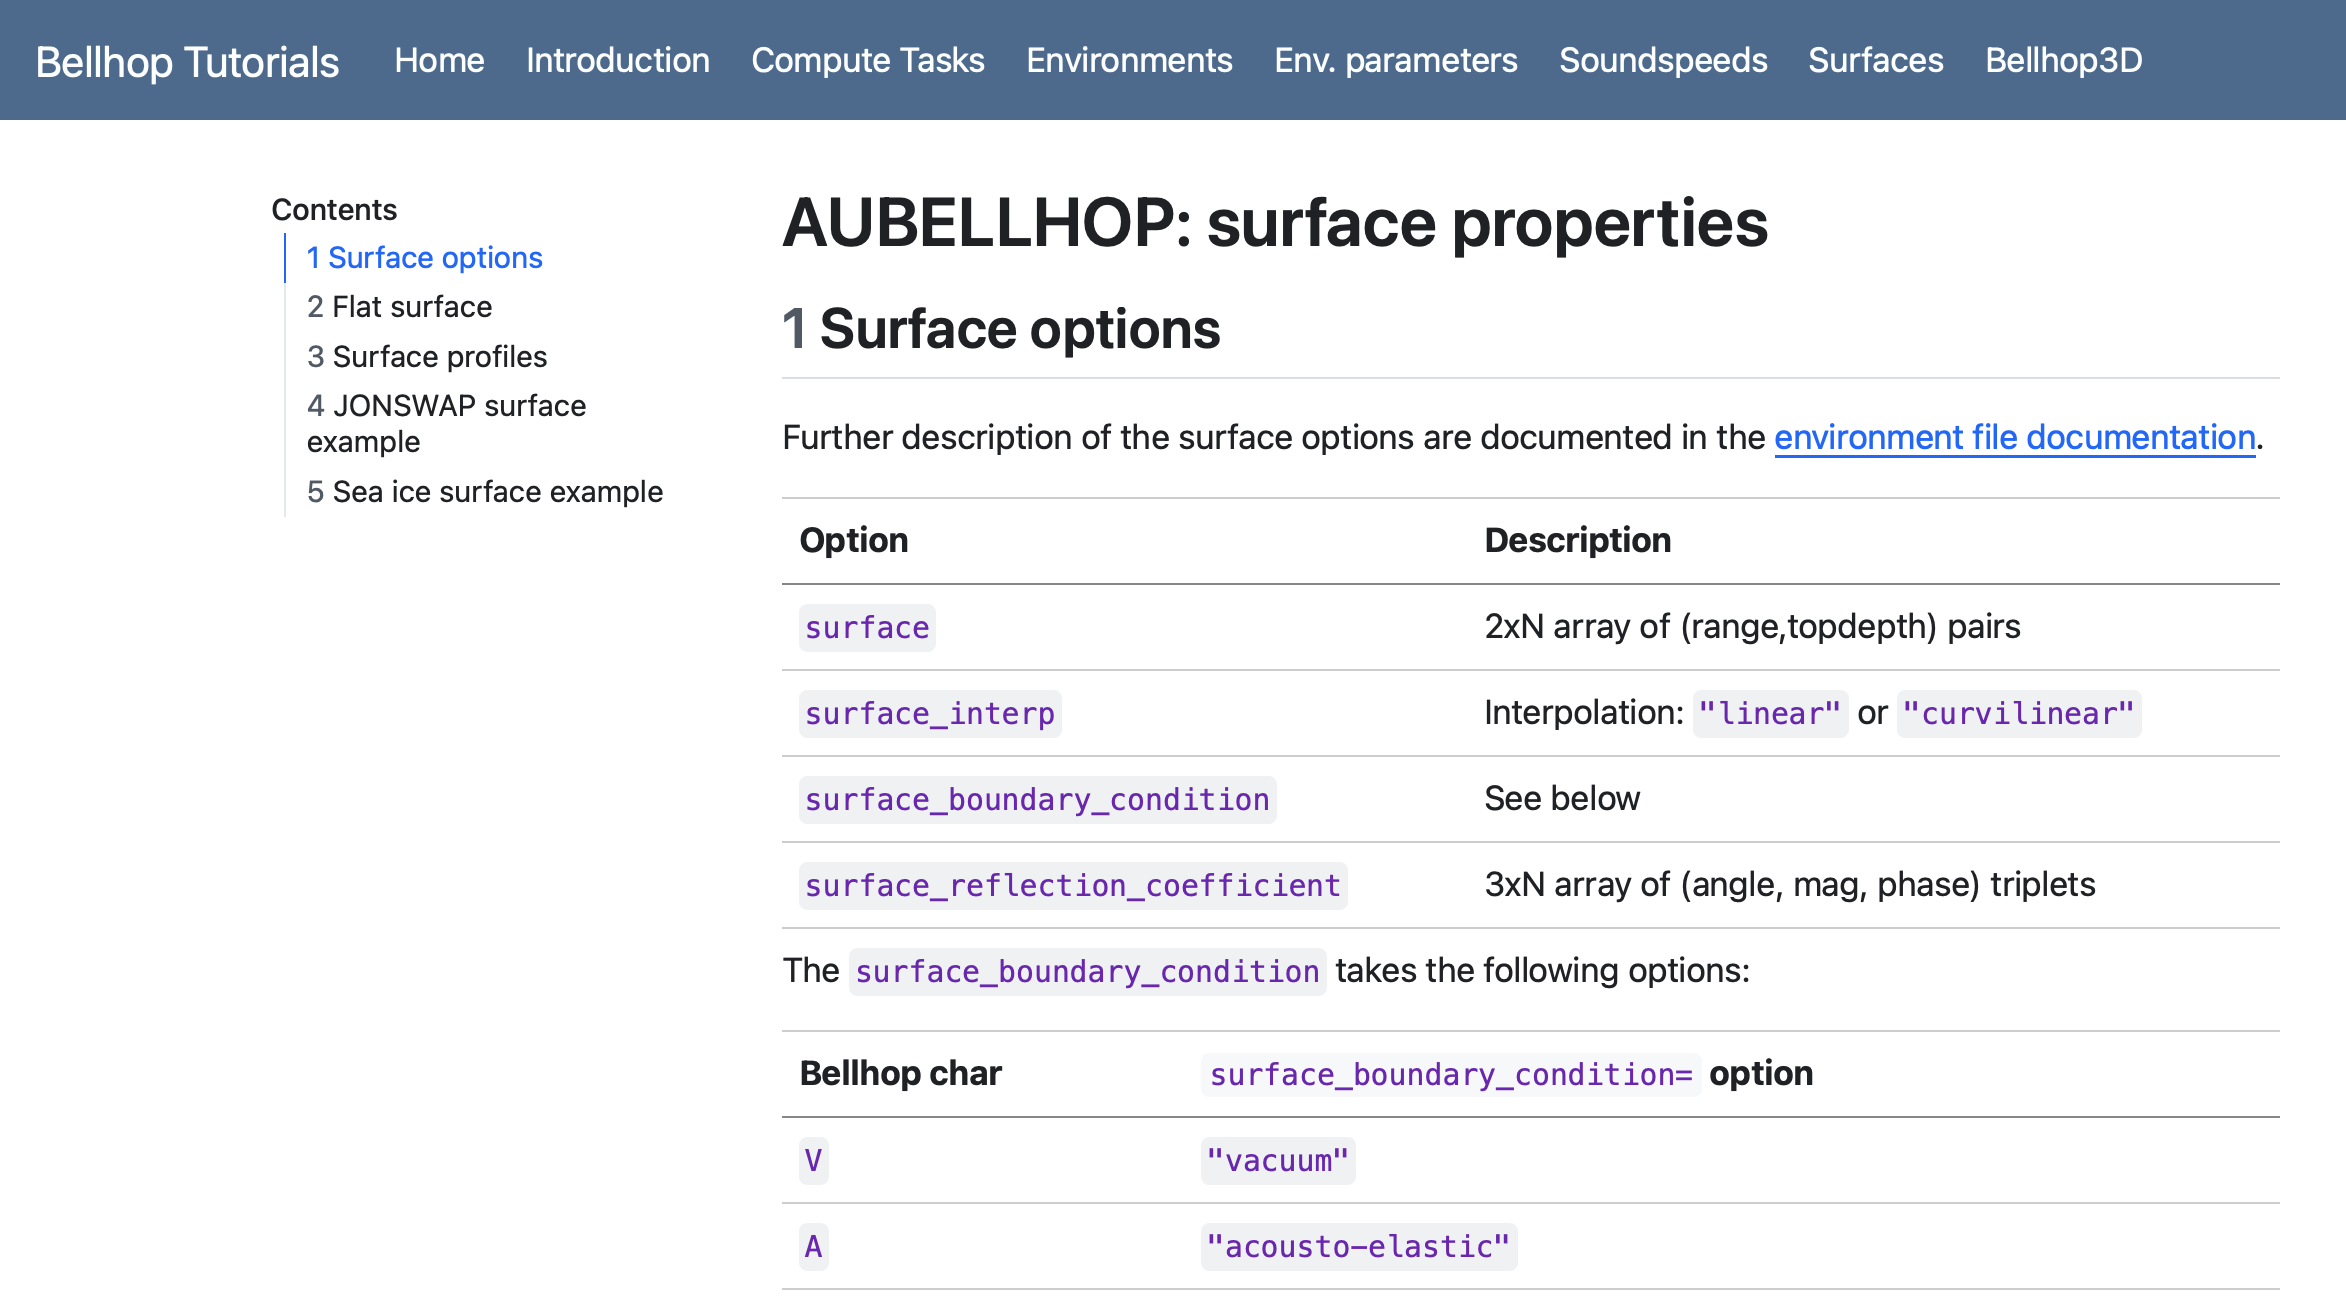
\includegraphics[width=0.8\linewidth]{fig/tute.png}
\caption{Screenshot of the \texttt{aubellhop} tutorials page.}
\figlabel{tute}
\end{figure}

\subsection{Using variable sound speed data}

An important consideration in underwater acoustics is the variable sound speed, which causes refraction of acoustic rays. The sound speed typically varies with depth due to changes in temperature, salinity, and pressure.
Bellhop (the executable) provides a number of interpolation routines for interpreting discretised sound speed data; some care should be used in ensuring that an appropriate interpolation is used.

In this example, we use sound speed data derived from the NOAA World Ocean Atlas by Brian Dushaw\footnote{\url{https://staff.washington.edu/dushaw/WOA/}}. A world-wide horizontal slices of this data at constant depth is shown in \Figref{lev_ssp}, with a vertical slice for constant longitude shown in \Figref{lev_ssp_long}. The code to perform the data manipulation into Python DataFrame format is not interesting here (see the repository page for a worked example), but once this is set up an example eigenray analysis with 2D sound speed data can be undertaken as follows:
\begin{verbatim}
env = bh.Environment( soundspeed=svp,
  bottom_depth=5500, source_depth=2000,
  receiver_depth=1000, receiver_range=40_000 )
erays = bh.compute_eigenrays(env)
bhp.pyplot_rays(erays, env=env)
\end{verbatim}
The eigenrays exhibit the typical refraction and focussing behaviour seen in deep ocean acoustic wave propagation due to the varying speed of sound (\Figref{lev_ssp_rays}).

\begin{figure}
\centering
\includegraphics[scale=0.9]{fig/lev_ssp.pdf}
\vspace*{-\baselineskip}
\caption{Sound speed profile (constant depth \qty{300}{m}), from NOAA World Ocean Atlas data.}
\figlabel{lev_ssp}

\centerline{\includegraphics[scale=0.9]{fig/lev_ssp_long.pdf}\quad\includegraphics[scale=0.9]{fig/lev_ssp_chk.pdf}}
\vspace*{-\baselineskip}
\caption{Sound speed profile for constant longitude \ang{200.5}.}
\figlabel{lev_ssp_long}

\centering
\includegraphics[scale=0.9]{fig/lev_ssp_rays.pdf}
\vspace*{-\baselineskip}
\caption{Eigenray analysis between a source and receiver with a 2D sound speed profile.}
\figlabel{lev_ssp_rays}
\end{figure}

\subsection{Using altimetry data}

The concept of this example was heavily inspired by the work of \textcite{alexander2013-aa}.
Surface profile data was extracted from a database of submarine upwards looking sonar data from the National Snow And Ice Data Center \cite{nsidc1998-ice}.
A section of this data was extracted directly from the source files of the database (file \texttt{2000a-000b-uwa.series}) and shown in \Figref{ice}.
Altimetry data of this sort can be used to define surface profiles for Bellhop:
\small
\begin{verbatim}
env = bh.Environment(
    source_depth=20,  bottom_depth=50,
    surface_depth=ice_data, # see code for details
    surface_boundary_condition="acousto-elastic",
    surface_soundspeed=3500, surface_density=890,
    surface_attenuation=0.4,
    attenuation_units="dB per wavelength",
    beam_num=20, beam_angle_min=-45, beam_angle_max=45,
)
\end{verbatim}
\normalsize
As the reflections off the ice are not governed by standard `vacuum' boundary conditions, addition settings are provided to capture these behaviours correctly.
The impact of the scattered reflections is shown in transmission loss contours (\Figref{ice-tl}) for \qty{400}{Hz} coherent reflections, \qty{20}{mm} grid spacing.
Although not intended to illustrate a substantive scientific conclusion, it is interesting to see the potential challenges that may be faced trying to predict or estimate acoustic properties in such environments.

\begin{figure}
\centering
\centerline{\includegraphics{fig/ice.pdf}
\includegraphics{fig/ice-rays.pdf}}
\caption{Artic ice profile from upwards looking sonar data (left); ray propagation for a region of the ice sheet (right).}
\figlabel{ice}

\centerline{\includegraphics{fig/ice-tl.png}
\includegraphics{fig/ice-tl-flat.png}}
\caption{Using measured ice profile data to calculate transmission loss (left), compared to a smooth ice surface (right). The source is at a depth of \qty{20}{m}.}
\figlabel{ice-tl}
\end{figure}


\section{Development details}
\label{sec:code}

Bellhop is an example of a long-standing open source software package that has enabled a large body of additional research to be built upon the foundation it provides.
It makes for an interesting case study to discuss open science, as it is currently published openly, and widely used by the research community, with an ecosystem of tools that have been built to interface with it.
Nonetheless, it is a `legacy' codebase in the sense that it is reliable and stable, and as a result does not make use of modern software development practices.
The following key additions were undertaken to modernise the Bellhop codebase.

\paragraph{Automatic code documentation, including dependency graphs}

There are several widely-used automatic code documentation tools, including Doxygen and Sphinx.
Because Bellhop is written in Fortran, the FORD tool was selected to generate its base documentation.
Only minor changes to the Bellhop Fortran sources were needed for the comments in the file to match FORD's expectations.
A modified comment prefix (\verb|!!|) creates specially tagged documentation strings that are extracted for the summary online documentation (\Figref{ford-modules}), which presents an overview of the collections of files, modules, procedures, and so on, in the codebase.

FORD analyses the code and creates connected graphs (\Figref{graphvis}) to link files to files, modules to modules, and so on. Most importantly, this showed which source files were not being used in the Bellhop codebase, as it is provided in its original form alongside additional underwater acoustics programs -- Kraken, etc.\ -- with a shared library.

The Python interface to bellhop is documented using Sphinx (following arlpy). The Sphinx output is combined with the main FORD output to create the documentation pages.

\paragraph{Regression and unit testing suite}

Engineering software is uniquely well-suited to many types of testing approaches, as numerical outputs can be explicitly queried.
For Bellhop, the Acoustics Toolbox distribution contains a very large number of examples, which allows verification testing that any changes to the source files do not result in execution failures.
However, these examples do not attempt to perform validity checks that their numerical output is correct.
Introducing a Python-based testing procedure was critical in being able to make changes to the Fortran sources with confidence.
The Python-focussed tests ensure that interfaces are consistent with the legacy Bellhop input files, that complex environment configuration parameters are being correctly implemented, and that post-processing and visualisation data routines are operating as specified.
At time of writing there are 35 test files, covering 192 unique tests.

Even with good intentions to write tests as the code is written, it is difficult to manually assess whether a test suite actually checks all possible code paths of a program.
Without feedback about what is being tested, we cannot independently verify that we have enough tests.
`Code coverage' reporting is an automated approach to identifying how much of the source code is being executed when the test suite runs (\Figref{coverage}, left).
A source file with less than 100\% coverage is likely to have branches which are not being tested; for instance, this often occurs when a feature is provided with a range of options, and not each option is explicitly tested (\Figref{coverage}, right).



\paragraph{Coding standards (lint and type checking)}

Modern `lint' tools such as \verb|ruff| (for Python) and \verb|fortitude| (for Fortran) are designed to enforce coding standards.
Code written to standard are less likely to contain subtle bugs, and minimise friction moving between codebases.
E.g., developers experience friction when there are inconsistencies with something trivial like spaces, or not, around maths operators.
When coded to standards, a new contributor does not face having to adapt to another developer's personal style.

When first used on the Bellhop repository, \verb|fortitude| reported 1168 `errors'.
These include trivial issues such as trailing whitespace in source code, long lines of code, deprecated operators, hard-coded numeric values, and so on.
To be clear, these 1168 so-called errors are not indicating there are any problems with the Bellhop code, nor that its developers were taking shortcuts in the development.
Modern linter tools by default are strict about upholding what are now considered to be best practice guidelines, but which may not have been (or could not have been) rigorously followed in years past.

\paragraph{Easy build systems}

Traditional workflows used \verb|make|, and modern Python tools such as \verb|uv| provide more complex environment setup options.
The Bellhop repository is set up with UV used for running the main development tools, with a transparent user interface provided by Make to help streamline shifting from one build process to another in the future.
The Make interface is as simple as (\verb|make help|):
\begin{verbatim}
CODE BUILDING                          CODE CHECKING
  [all] - default: build binaries           test - run test suite
  clean - remove all temporary files   cleantest - rebuild codebase, run tests
install - copy binaries into ./bin          lint - run code linters
                                             doc - build online documentation
                                             cov - run code coverage processes
\end{verbatim}

\paragraph{Online repository hosting}

This project is hosted on Github, likely the most popular online code repository at time of writing.
Github provides generous support for educational and open source users.
A publicly hosted project provides a stable home to access the work, but online platforms offer many desirable features, including collaboration and project management tools (such as pull requests and issue tracking), ability to serve websites based on project documentation, and so-called `continuous integration' workflows.
Very recently (at time of writing), it is now possible to integrate AI agents into online repositories, who can run, analyse, and suggest changes to code directly.

As part of the online repository, a comprehensive suite of documentation is being written, which covers the Fortan code and interfaces, the \texttt{aubellhop} code and interfaces, and a set of tutorials demonstrating common use cases.
The accessibility of this modern documentation is intended to allow new uses to adopt Bellhop easily using free, open source workflows.

\begin{figure}
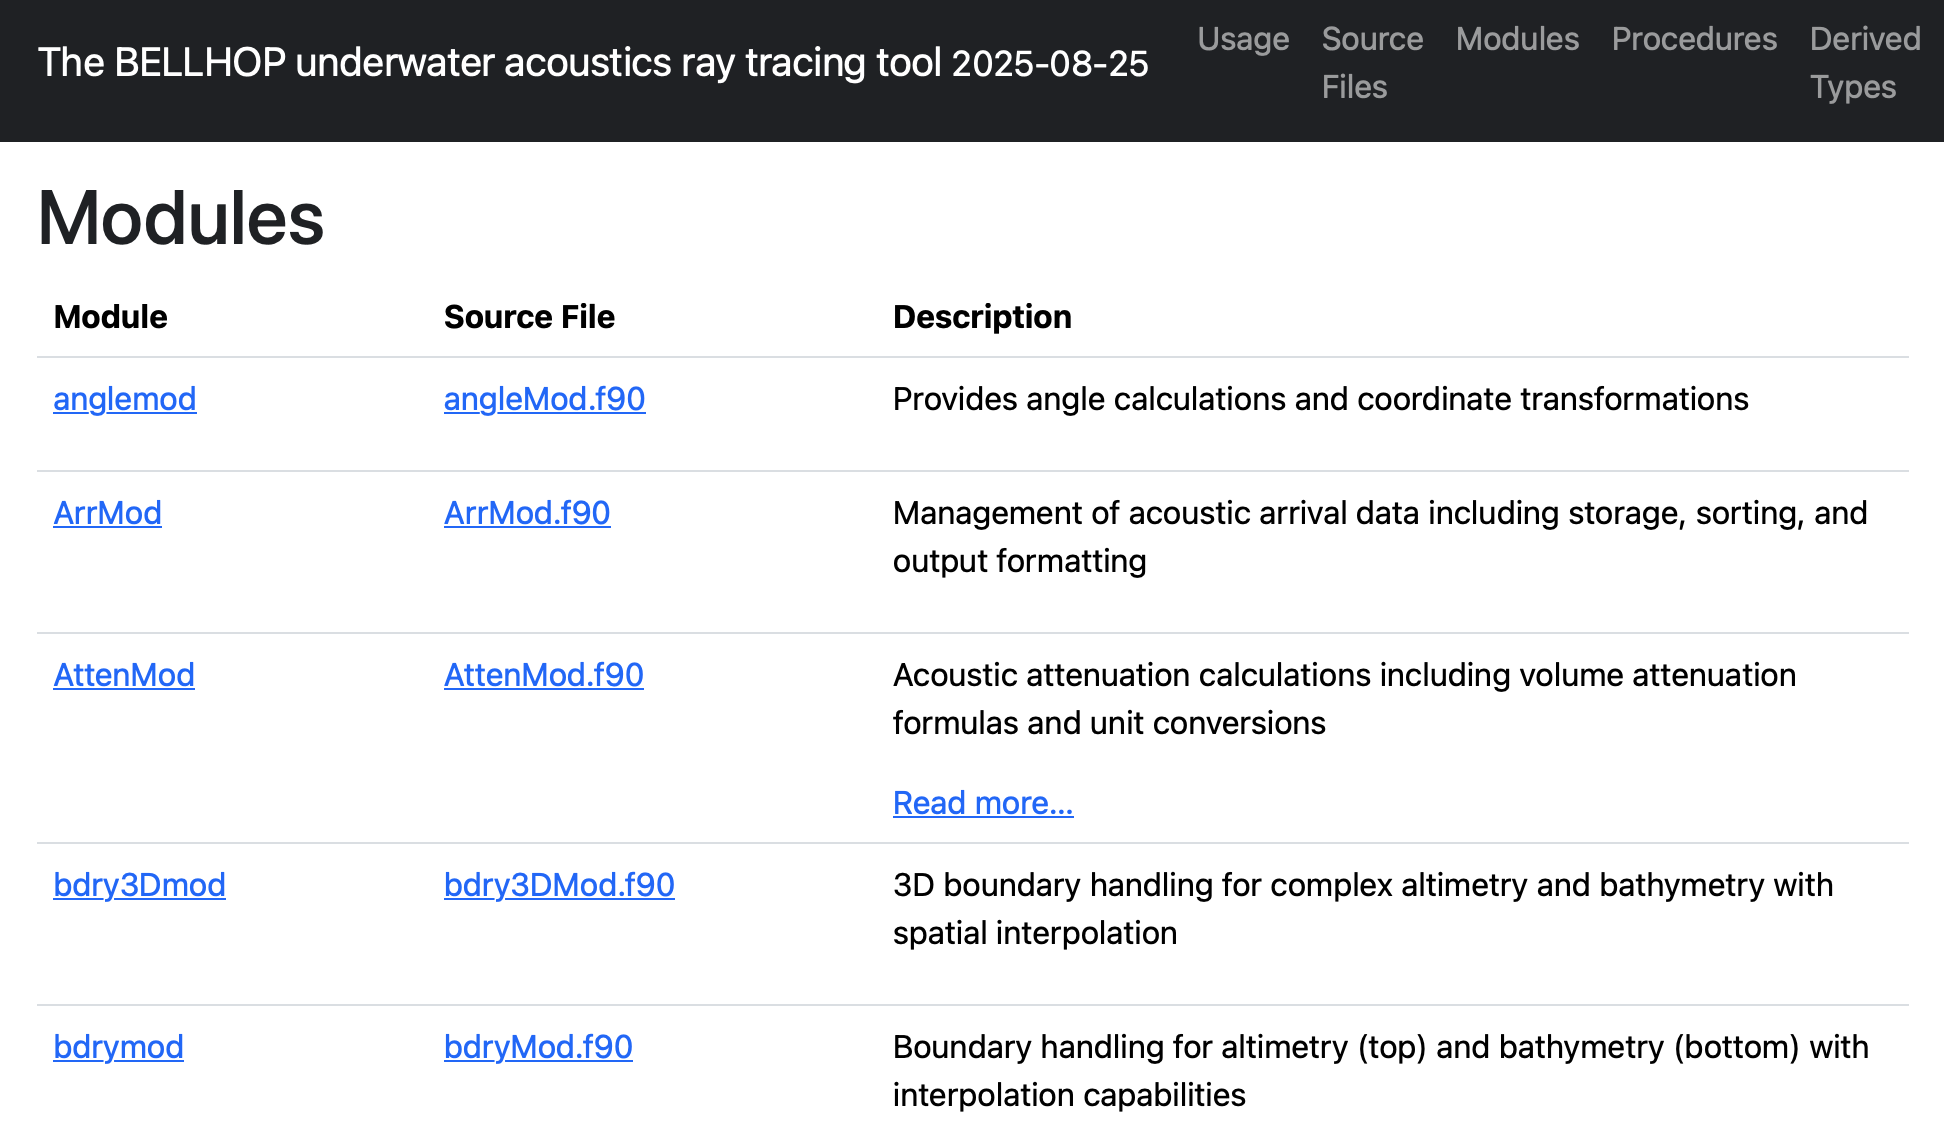
\includegraphics[width=0.45\linewidth]{fig/ford-modules-snap.png}\hfil
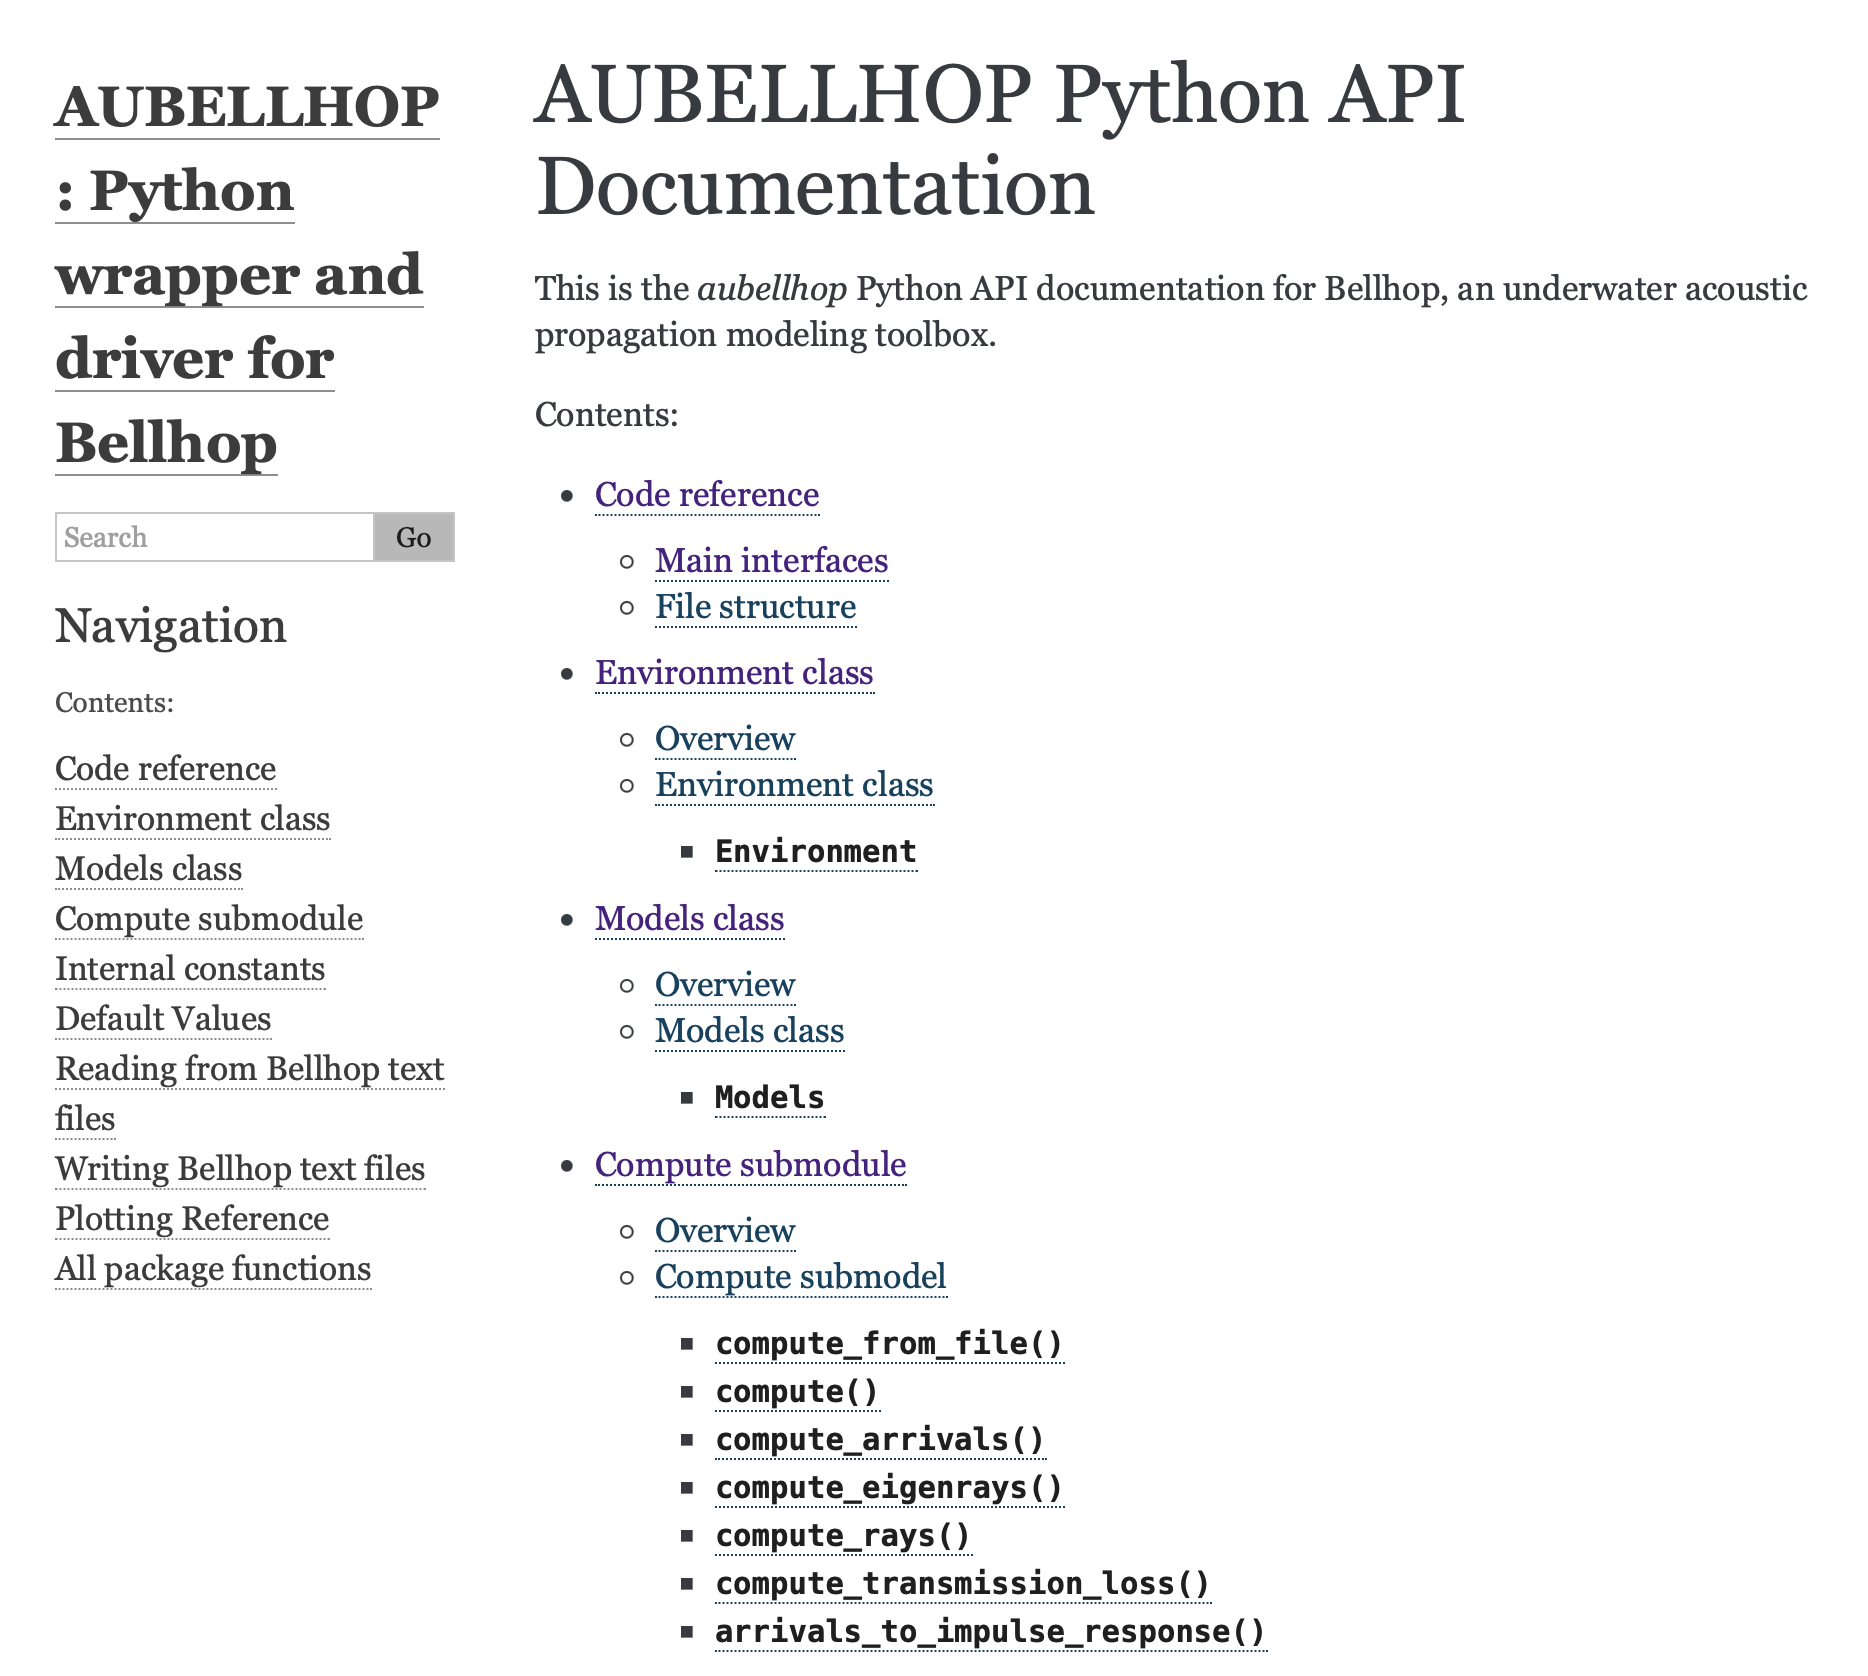
\includegraphics[width=0.45\linewidth]{fig/api}
\caption{Example output of the FORD Fortran Modules documentation (left) and the Sphinx Python API documentation (right).}
\figlabel{ford-modules}
\bigskip

\centerline{\fbox{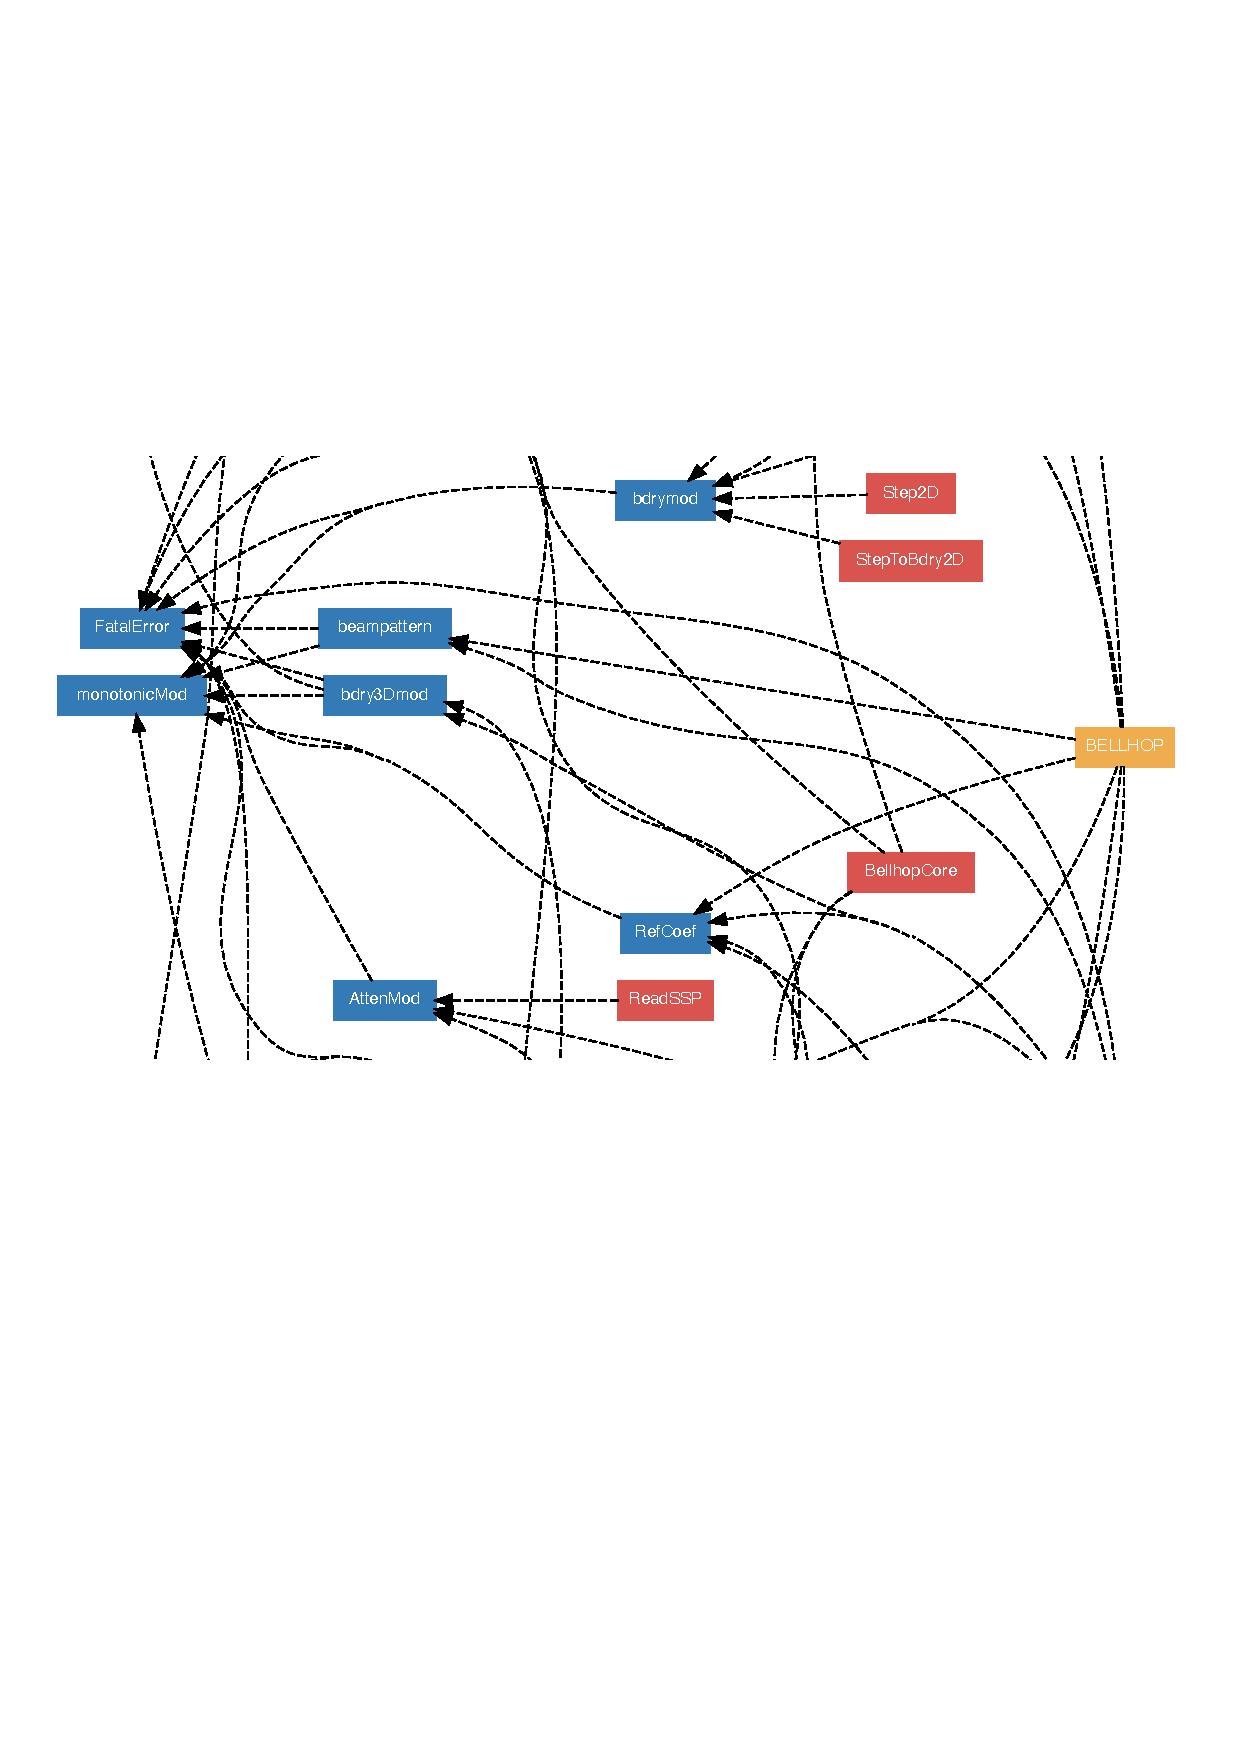
\includegraphics[width=0.8\linewidth]{fig/graphvis}}}
\caption{Extract from part of the automatically-generated Graphvis output from the FORD Modules documentation.}
\figlabel{graphvis}
\bigskip

\centering
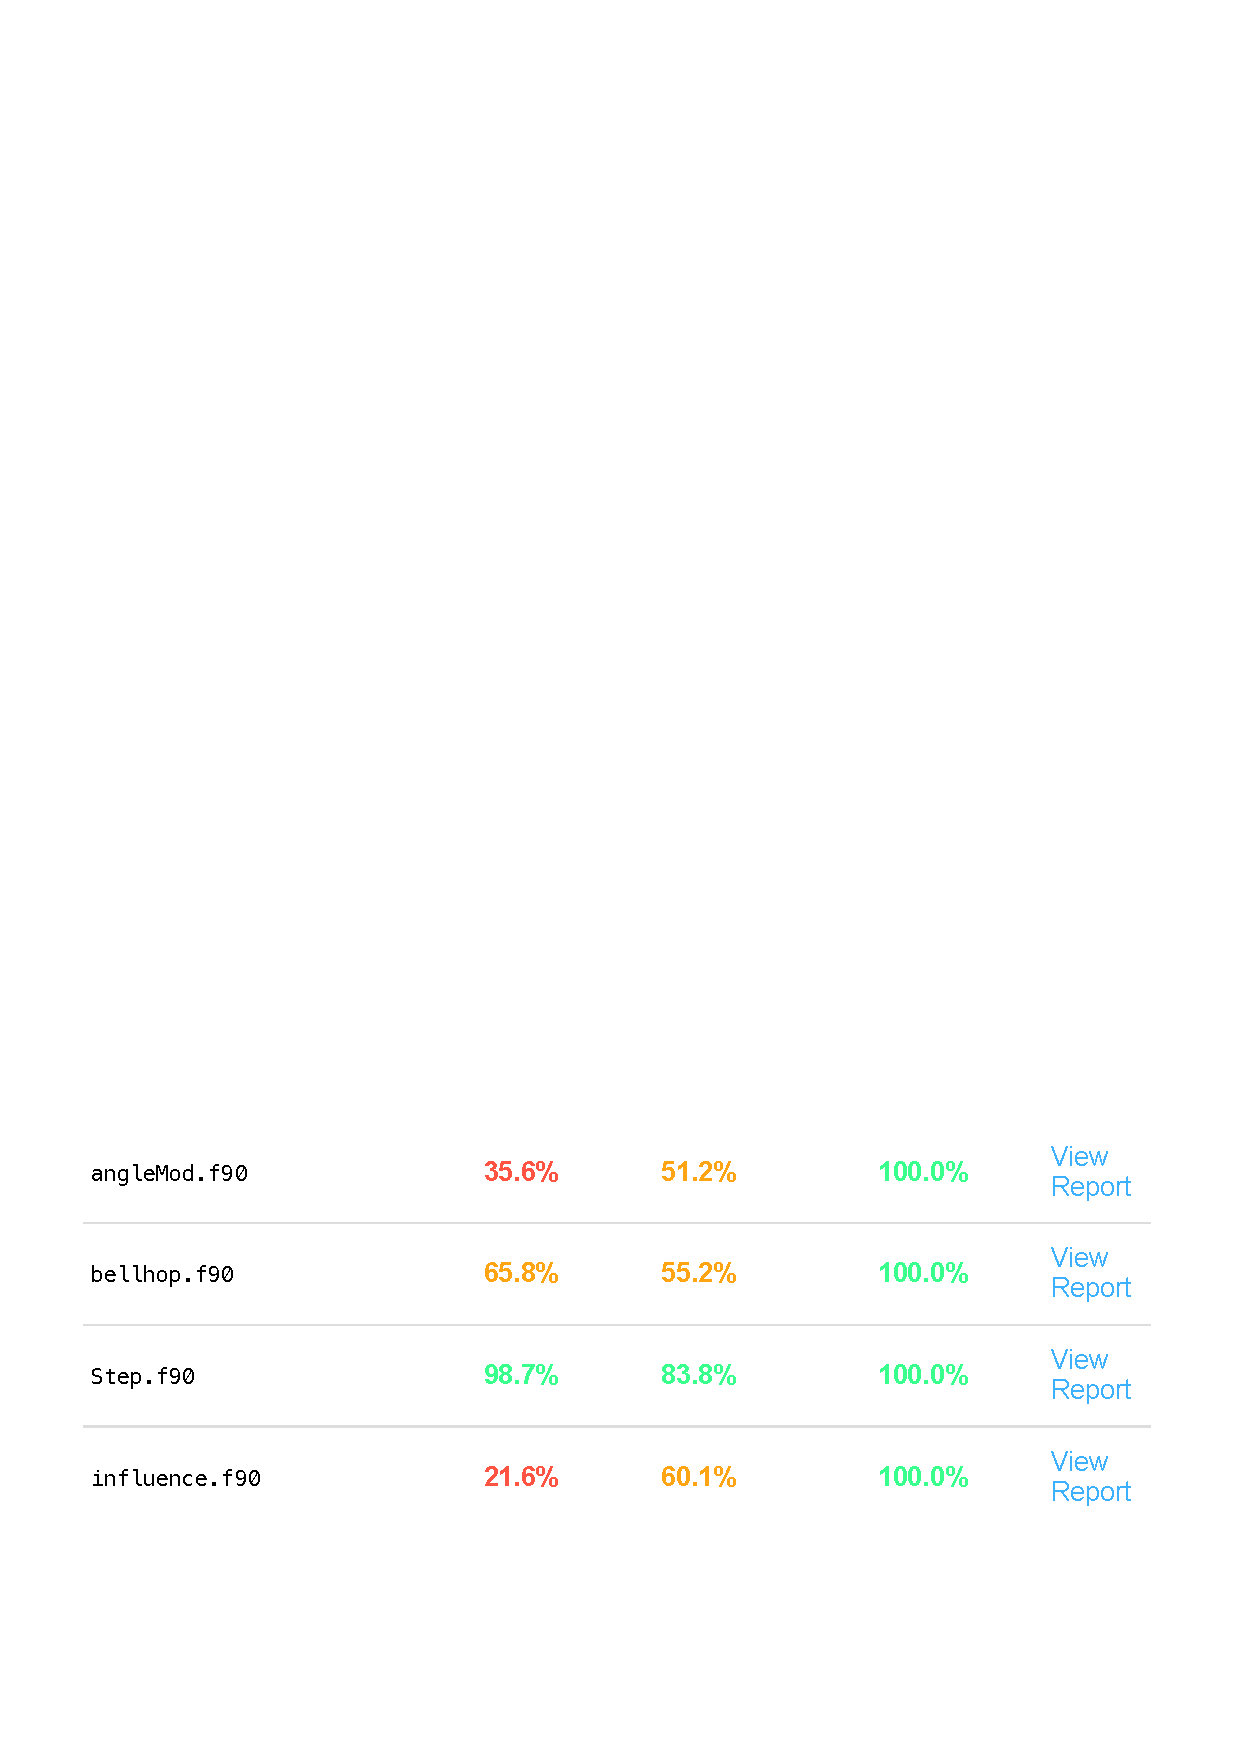
\includegraphics[width=0.45\linewidth]{fig/coverage.pdf}\hfil
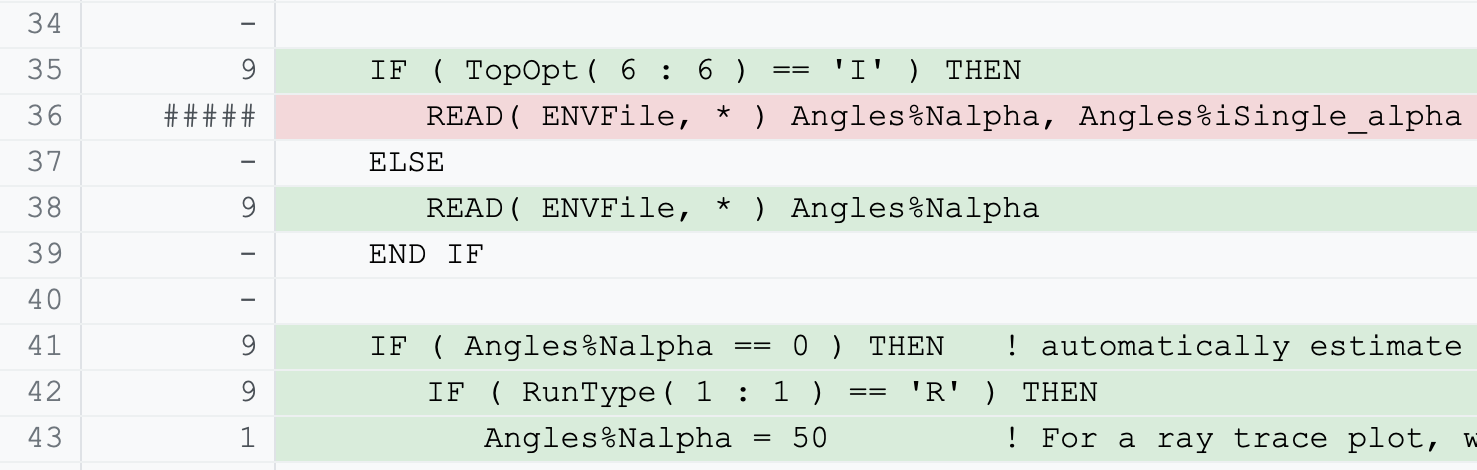
\includegraphics[width=0.45\linewidth]{fig/cov-detailed}
\caption{Example of coverage report summary output (left) and detailed per-file output (right). Each file contains a detailed report that shows the number of times each line of code is executed by running the test suite. In the detailed output, the red highlight shows code which is not run as part of the test suite.}
\figlabel{coverage}
\end{figure}


\section{Conclusion}
\label{sec:conclusion}

Bellhop retains its research potential some forty years after its first release, and we hope that by making this codebase more accessible it will provide easier access to this valuable tool by underwater acousticians and researchers.
Building engineering software using these features helps mitigate the risk of unknown errors in the code, promotes reproducibility, and largely comes `for free' using modern programming tools and libraries.

This work builds off \texttt{arlpy} to provide a user-friendly interface to Bellhop in Python. Extensions to \texttt{arlpy} in \texttt{aubellhop} include streamlining of the main interfaces, adding additional features associated with data processing and plotting, and providing further interfaces to the underlying Bellhop executable(s).
Future work will involve testing against the \texttt{bellhopcuda} executables, expanding support for 3D data visualisation, and building parallelisation into the interface.

As beam- and ray-tracing algorithms are inherently sensitive to their modelling conditions, providing well-tested and reproducible development environments for simulation work is critical to ensure that results are meaningful and verifiable.
We thank the authors of Bellhop and its peers for the substantial contributions they have made to the acoustics community in sharing their work openly, and trust that there will be many decades of further evolution of these tools.

\clearpage
\printbibliography

\end{document}

